% use "amsart" instead of "article" for AMSLaTeX format
\documentclass[a4paper,11.5pt]{report}   
\renewcommand{\baselinestretch}{1.5} 

\usepackage[strings]{underscore}
\usepackage{datetime}

\newdateformat{monthyeardate}{%
  \monthname[\THEMONTH], \THEYEAR}

\usepackage{enumerate}

\usepackage{setspace}

%\usepackage[margin=1.2in]{geometry}

\usepackage[a4paper,bindingoffset=0.4in,%
            left=1in,right=1in,top=1in,bottom=1in,%
            footskip=.25in]{geometry}
            


% ... or a4paper or a5paper or
\geometry{a4paper}      
             		
% Activate to begin paragraphs with an empty line rather than an indent
\usepackage[parfill]{parskip}   

 % Use pdf, png, jpg, or eps§ with pdflatex; use eps in DVI mode		
\usepackage{graphicx, wrapfig}				

\setcounter{secnumdepth}{4}

\usepackage{nomencl}
\makenomenclature

\usepackage{lipsum}

\usepackage{gensymb}

%\usepackage[monochrome]{color}
%\usepackage[utf8]{inputenc}


\usepackage{float}

\usepackage{amsmath}
	\numberwithin{figure}{section}
	\numberwithin{table}{section}
	\numberwithin{equation}{section}

\usepackage{amsmath}
	\numberwithin{equation}{section}
	\newcommand*{\Scale}[2][4]{\scalebox{#1}{$#2$}}%
	
\usepackage{multirow}

\usepackage{appendix}

\usepackage{array}

%\newcolumntype{P}[1]{>{\centering\arraybackslash}p{#1}}

\usepackage{blindtext}

\usepackage[export]{adjustbox}[2011/08/13]
	
\usepackage{gensymb}
	
\usepackage{colortbl}

\usepackage{longtable}

\usepackage{tabularx}

\usepackage{enumerate}

\newcommand{\gray}{\rowcolor[gray]{.90}}

\makeatletter
\newcommand*{\rom}[1]{\expandafter\@slowromancap\romannumeral #1@}
\makeatother

\usepackage{rotating}

%\bibliographystyle{unsrtnat}
\usepackage{natbib}
\newcommand*{\urlprefix}{Available from: }
\newcommand*{\urldateprefix}{Accessed }
\bibliographystyle{bathx}
%\usepackage[sort&compress,numbers]{natbib}


\usepackage[final]{pdfpages}

\usepackage{caption}

\usepackage[% line break after label
   singlelinecheck=off, font=bf]{caption}
%\newcommand{\rom}[1]{%
%  \textup{\expandafter{\romannumeral#1}}%
%}

\usepackage{tocloft}
\renewcommand{\cftpartleader}{\cftdotfill{\cftdotsep}} % for parts
\renewcommand{\cftchapleader}{\cftdotfill{\cftdotsep}} % for chapters
 \renewcommand\cftchapafterpnum{\vskip10pt}

 
%\usepackage{titletoc}% http://ctan.org/pkg/titletoc
%\titlecontents*{chapter}% <section-type>
%  [0pt]% <left>
%  {}% <above-code>
%  {\bfseries\chaptername\ \thecontentslabel.\quad}% <numbered-entry-format>
%  {}% <numberless-entry-format>
%  {\bfseries\hfill\contentspage}% <filler-page-format>


\usepackage{subfig}					%use figure packagesx

\makeatletter

\newcommand\frontmatter{%
    \cleardoublepage
  %\@mainmatterfalse
  \pagenumbering{Roman}}

\newcommand\mainmatter{%
    \cleardoublepage
 % \@mainmattertrue
  \pagenumbering{arabic}}

\newcommand\backmatter{%
  \if@openright
    \cleardoublepage
  \else
    \clearpage
  \fi
 % \@mainmatterfalse
   }

\makeatother

\usepackage{fancyhdr}
\fancyhf{}
  \fancyhf[lef,rof]{\thepage}%
\pagestyle{fancy}
\fancypagestyle{plain}{%
  \fancyhf{}%
  \renewcommand{\headrulewidth}{0pt}%
  \fancyhf[rof]{\thepage}%
}

\usepackage{memhfixc}

\renewcommand{\contentsname}{Table of Contents}

\usepackage{pdflscape}

\usepackage{lscape}

\usepackage{textcomp}

%\usepackage[libertine,cmintegrals,cmbraces,vvarbb]{newtxmath}

%\usepackage[sorting=none]{biblatex}

\usepackage{notoccite}

\usepackage{titlesec}
\usepackage{appendix, apptools}
\AtAppendix{%
\titleformat{\chapter}[display]{\vspace*{-30pt}\bfseries\huge}{\chaptername~\thechapter}{1em}{}
\titlespacing*{\chapter}{0pt}{0pt}{0pt}}%

\makeatletter
\newcommand{\mypm}{\mathbin{\mathpalette\@mypm\relax}}
\newcommand{\@mypm}[2]{\ooalign{%
  \raisebox{.1\height}{$#1+$}\cr
  \smash{\raisebox{-.6\height}{$#1-$}}\cr}}
\makeatother

\usepackage{afterpage}
\newcommand\blankpage{%
    \null
    \thispagestyle{empty}%
    \addtocounter{page}{-1}%
    \newpage}
    
\usepackage{url}


%\title{
%Development an Educational Game to Teach SQL Programming
%}
%\author{
%Amarnath Kakkar \\
%\normalsize University of Bath
%}
%\date{}							% Activate to display a given date or no date


\begin{document}

\frontmatter


%titlepage
\clearpage\thispagestyle{empty}
\begin{center}
\begin{minipage}{0.9\linewidth}
    \centering
%University logo
    \vspace{0.8cm}
    
\includegraphics[width=0.4\linewidth]{logobath.jpg}\par
    
    \vspace{2.5cm}
%Thesis title
    \vspace{0.2cm}
    {\uppercase{\Large \textbf{Development of an Educational Game to Teach Iteration and Conditional} \par}}
    \vspace{3cm}
%Author's name
    {\Large \textbf{Amarnath Kakkar}\par}
        \vspace{3cm}
% $^{\circ}$
    {\large A final year project submitted in partial fulfilment for the degree of Bachelor's in Computer Science and Mathematics with Honours\par}
    {\large University of Bath\par}
    \vspace{4.5cm}
%supervisor and date
    {\large \textbf{\monthyeardate\today}\par}
    \vspace{1cm}
\end{minipage}
\end{center}

\afterpage{\blankpage}




\clearpage\thispagestyle{empty}
\begin{center}
\begin{minipage}{0.9\linewidth}
%University logo

\vspace{10cm}
{This dissertation may be made available for consultation within the University Library and may be photocopied or lent to other libraries for the purposes of consultation.\par}
\vspace{1cm}
Signed: 
   	
	
\end{minipage}
\end{center}

\newpage



    
\clearpage\thispagestyle{empty}
\begin{center}
\begin{minipage}{1\linewidth}
%Thesis title
%    \vspace{0.2cm}
%    {\uppercase{\large {Submitted in partial fulfilment for the degree of masters in aerospace engineering} \par}}
    \vspace{2cm}
%%Author's name
    {\LARGE Development of an Educational Game to Teach Iteration and Conditional \par}
    \vspace{1cm}	
    {\large Submitted by: Amarnath Kakkar\par}
	
    \vspace{1.5cm}
    {\Large \textbf{COPYRIGHT}\par}
    \vspace{0.5cm}
    {Attention is drawn to the fact that copyright of this dissertation rests with its author. The Intellectual Property Rights of the products produced as part of the project belong to the author unless otherwise specified below, in accordance with the University of Bath?s policy on intellectual property
(see http://www.bath.ac.uk/ordinances/22.pdf).
This copy of the dissertation has been supplied on condition that anyone who consults it is understood to recognise that its copyright rests with its author and that no quotation from the dissertation and no information derived from it may be published without the prior written consent of the author.\par}

     \vspace{0.5cm}
     {\Large \textbf{Declaration}\par}
      \vspace{0.5cm}
      {This dissertation is submitted to the University of Bath in accordance with the requirements of the degree of Bachelor of Science in the Department of Computer Science. No portion of the work in this dissertation has been submitted in sup- port of an application for any other degree or qualification of this or any other university or institution of learning. Except where specifically acknowledged, it is the work of the author.\par}
    
     \vspace{2.5cm}
%% $^{\circ}$
    {\large Department of Computer Science\par}
    {\large University of Bath\par}
    \vspace{0.5cm}
%supervisor and date
    {\large Supervisor: Dr. Alan Hayes}\par
    {\large \textbf{\monthyeardate\today}\par}
    \vspace{1cm}
\end{minipage}
\end{center}

\afterpage{\blankpage}

\hfill

\section*{\Huge{Abstract}}

To be written.



\newpage

\addtocontents{toc}{\protect\setstretch{1}}
\tableofcontents

\newpage
{%
\let\oldnumberline\numberline%
\renewcommand{\numberline}{\figurename~\oldnumberline}%
\listoffigures%
}

\newpage
\listoftables  

\newpage
\hfill

\section*{\Huge{Outline of Project}}

To be written.

\newpage
\hfill
\section*{\Huge{Acknowldgements}}

To be written.
 
\afterpage{\blankpage}

\mainmatter

\chapter{Introduction}
\afterpage{\blankpage}

\chapter{Literature Review}
%\section{Aims of This Section}

%This Literature Review aims to bring together various studies, and provide an insight into the use of games for educational purposes. It also aims to critically evaluate the material for any consistencies or inconsistencies, and to hopefully provide another perspective on the field.

%\subsection{Defining Serious Games}
%In the area of gamification, various definitions of serious games are found. Most commonly, and perhaps quite broadly, the term 'serious game', is defined as, digital games used for purposes other than mere entertainment \cite{Susi2416}.  While a variety of definitions have been suggested, this dissertation will use the definition suggested by \cite{Garris2002} who saw it as "instructional games that are designed for training or to promote learning" together with "games that do not have entertainment, enjoyment or fun as their primary purpose"  \cite{MichaelChen2006}. However, it is not to say that serious games should not be entertaining, enjoyable or fun.

%\subsection{Outline of Review}
%This review will; identify the benefits of serious games, and make clear any negatives, go through examples of serious games and their approaches, including any specific game design elements implemented, and outline any techniques that seem to be of positive influence or negative influence, look into existing resources for teaching SQL and outline the trade-offs with each approach, finally bring together these ideas summarise various points.

%\section{Benefits of Serious Games}
%Today's students are brought up in the digital era. \cite{Prensky2001} refers to them as 'Digital Natives', that have experienced a new form of video game play, which brings opportunities with great potential for their learning. Thus potentially making games great learning environments within education. However, \cite{Girard2013} summarises that there is need for more empirical research to determine the effectiveness of serious games. On the other hand, \cite{Pieter2013} reports that in general, serious games are more effective than traditional teaching methods, and that more studies are required to determine the effects of various features.

%In this section, we will outline some of the empirical researches that exist on the internet.

%\subsection{}

%\section{Examples of Serious Games}
%\subsection{Game Design Elements}
%\section{Existing Methods for Teaching SQL}
%\section{Summary}
\section{Teaching Programming Fundamentals}

In 1978, ACM Computing Curricula used the terms "CS1" and "CS2" to designate the first two courses in the introductory sequence of a computer science undergraduate course. CS1 described introducing students to programming fundamentals and CS2 to teaching data abstraction/data structures. The general principles of CS1 and CS2 have continued, but through the past years, the concepts covered in these courses have changed. The most recent curriculum by ACM-IEEE was created in 2013 \citep{Hertz2010}. This curriculum notes that the "vast majority of introductory courses are programming-focused, in which students learn about concepts in computer science (e.g., abstraction, decomposition, etc.) through the explicit tasks of learning a given programming language and building software artifacts". The curriculum considers 'conditional and iterative control structures' as fundamental programming concepts \citep{acm}. Thus these concepts are likely be taught as a part of CS1 or introductory programming units. %CS course guidelines

%Computer Science departments in the UK and USA report declining enrollment and high attrition rates on their degree programs. Student attrition is exacerbated during and between the first and second years of these programs. These high attrition rates are associated with considerable failure rates in introductory programming courses. The changes to the computing industry associated with, inter alia, new technologies, and the problems associated with learning to program, have led to Higher Education Institutions facing the pressing need to rethink their CS curricula, with special attention given to redesigning the CS1 course.

\citeauthor{Koulouri2014} bring together literature and summarise, that, the complexity of teaching introductory programming, which includes the topics; iteration and conditional statements, is widely acknowledged among educators. Novice programmers have difficulty in tracing (a method of mentally simulating the execution of the code before compiling), reading and understanding pieces of code and fail to grasp basic programming principles and routines. The overhead of learning the syntax and semantics of a language at the same time, and difficulties in combining new and previous knowledge and developing their general problem-solving skills, all add to the complexity of learning how to program \citep{Koulouri2014}. Therefore careful consideration will be taken to reduce these problems, with efforts to; introducing programming concepts at a reasonable pace, and making the game fun and enjoyable to keep the user motivated. %Problems with teaching introductory programming to novices.

Introductory programming courses at University commonly entail, a structured course based on lectures and practical laboratory work, and a curriculum focused largely on programming knowledge - particularly relating to the features of the programming language being taught and how to use them. \citeauthor{Robins2003} suggest that this approach is popular, due to the important role of such programming knowledge in programming and the sheer volume and detail of language related features that can be covered \citep{Robins2003}.

Another method for learning programming fundamentals, which has become increasingly popular, are online resources. These resources include; tutorial websites such as Codeacademy and Khan Academy, which have accumulated millions of users; block-based programming environments such as Scratch and Alice, which provide creative visual environments, and educational games \citep{Lee2015}. 

In comparison, traditional face-to-face classroom learning, centers on instructors who have control over class content and the learning process, whereas, online learning, offers a learner-centered, self-paced learning environment. Online resources are also time and location flexible and provide unlimited access to learners \citep{Zhang2004}. On the other hand, whilst there are many benefits to online learning, there are doubts over its effectiveness \citep{Zhang2004}. Online learning should not replace traditional forms of learning \citep{Zhang2004, Gunasekaran2002, agal2010}, however using online learning to complement the learning process in academia, could improve the quality of the learners education \citep{Concannon2005, Zhang2004}.

\section{Video Games}

%The academic study of games, ludology, is a relatively new and emerging field. As the video game revolution took off in the late 20th century, so did academic interest in games. 

%Video games for entertainment have dominated the market, 

%The academic study of games, is a relatively new and emerging field. Games are naturally creative things, however academics see the potential in games for a variety of different reasons, and so game design frameworks have been developed to help design and create games.

The video games industry has grown very rapidly in recent years, and is expected to continue to grow. The current value of the market is predicted as \$150 billion USD and is expected to reach \$180 billion by 2022 \citep{vgamesResearch}. In 2006, video games were considered as one of the most popular forms of entertainment in the United States \citep{sherry2006, ritterfeld2006}. Now video games can be considered a popular form of entertainment globally.

A video game can be defined as "a mental contest, played with a computer according to certain rules for amusement, recreation, or winning a stake" \citep{Zyda2005}.

%Military applications have dominated the market, but civil applications are expected to grow [8][9]. UAV have already proved to be successful in field operations however, further research can enable UAV?s to be used in intelligence gathering, such as stealth and combat operations [34].

\subsection{History}

%The interest in UAV?s has been observed since 1916, when the first modern unmanned aircraft was invented, Hewitt?s UAV. This was a result of Sperry?s work, on the flight stabilisation using gyroscope devices, which provided flight stabilisation [11]. This attracted the interest of the US Navy however, due to technical difficulties the research and work in automatic planes was lost. In 1933 the Royal Navy Queen bee?s target drone was operated for the first time and the potential of UAV?s was understood, but it still required perfection of remote operations. Reginald Denny then developed the successful target drone RP-2, during WWII using radio control [12].

The earliest documented predecessor to video games was observed in 1948, when the "Cathode-Ray Tube Amusement Device" was patented. The amusement device, required players to overlay pictures of targets such as airplanes in front of the screen \citep{TennisForTwo}.

10 years later, physicist William A. Higinbotham was credited for creating the first video game; attempting to display his research at an exhibition, he anticipated that his display would not generate any interest, so he conceptualised and created 'Tennis for Two' \citep{historyVideoGames}. Tennis for Two was created using an analog computer with an oscilloscope for a screen. It was the first game to display motion and allow multiple players to play together \citep{TennisForTwo}. 

%Computer games are defined as games that are played on Personal Computers, and video games as games played using a television and a games console \cite{Cummings07}.

%In 1958, Tennis for Two was created using an analog computer and oscilloscope for a screen. Four years later, Spacewar was developed using a digital minicomputer and a cathode-ray tube as the display, making it one of the first computer games. In 1972, Computer space and Pong were among the first video games. They were played on televisions placed in upright cabinets, and this paved the look and feel for future arcade games \cite{TennisForTwo, Lowood2009}.

The rise of modern generation of video games is credited to the development of 'Spacewar!' in 1962, 'Computer Space' in 1971 and 'Pong' in 1972. Spacewar! was developed for academic purposes to test the limits of new hardware, but shortly after became very popular. Spacewar! was played by Nolan Bushnell, who used the idea of the game to create Computer Space, although, Computer Space did not gain much popular traction. This was partly due to its long winded instructions and complex game controls. Learning from these mistakes, the creators of Computer Space decided to create a simpler game and came up with the idea for Pong, which became very popular. Computer Space and Pong were designed solely for entertainment, and Pongs popularity was credited to the simplicity of its design \citep{Lowood2009}.


%The rise of modern generation of video games was a through the development of 'Spacewar!' in 1962, 'Computer Space' in 1971 and 'Pong' in 1972 \cite{Hector2003}. These video game were designed solely for entertainment \cite{Jean}. Spacewar! defined the main streams of computing research. Computer space did not gain traction, due partly to its long winded instructions and complex game controls, and so learning from these mistakes, the creators of Computer Space created the popular game 'Pong', and Pong's triumph was credited to the simplicity of its design \cite{Lowood2009}.

In the late 1980s, video games became a mainstream media industry \citep{Dmitri2003}.

\subsection{Impacts}

Initially the majority of research on the effects of playing games focused on the negative impacts; the potential harm related to violence, addiction and depression. But more recently studies have looked into their potential benefits \citep{Granic2014, Boyle2011, Ryan2006}.

Games provide a learning environment. Players first learn the rules of the game and the controls, then use this newly acquired knowledge to complete objectives and/or pass levels. In most games, the objectives get harder to reach as you progress, in turn testing the players knowledge and skill, and requiring increasingly complex solutions. Vygotsky claims that in these situations, progress is made when learners are presented with tasks which are just beyond their current level of ability \cite{}.

The research on the impacts of games is vast, so for the purpose of this dissertation, we will look at the benefits and drawbacks of educational games, which will be covered later on.

\subsection{Uses}

Video games now are used for a wide variety reasons, including in the following industries; military, government, education, corporate and healthcare, and also entertainment. The former set of industries for which games are created, that are not simply for entertainment, fall under the term 'Serious Games' \citep{Johann2015}.

%Many attempts to pinpoint the creation of the very first video game have been made. However, the creation of the first modern video game is commonly dated to 1958. first video game ever invented was developed by a physicist William Higinbotham, in 1958. The game was called 'Tennis for Two'. The design and concept was conjured up from an instructional book the inventor was reading at the time \cite{TennisForTwo}.

%The first recorded video game invented, was developed by a physicist called William Higinbotham, called 'Tennis for Two' in 1958. The concept of the game, came from an instructional book that he was reading at that time \cite{TennisForTwo}.

%In 1970, R. Barton discusses the evolution of 'The Imaginit Management Game' and the development of a game model. This model consisted of a set of rules, such that a management game could be repurposed to fit another management scenario \cite{Barton1970}.

%First a set of generality aspirations were defined, and then a set of strategies 'describes features of "generalized" management computer game and then reports a case history of adapting this game model, which was designed for ideal generality, to an application that challenged that very generality.

%\section{Benefits of Video Games}

%\subsection{Platforms}

\section{Educational Games}

Educational games form a subset of serious games \citep{Michael2005, Zyda2005}. The market value of serious games industry in 2010, was predicted as 1.5 billion EUR. The study of serious games become an established academic field, evidenced by the founding of The Serious Games Institute at Coventry University in 2007 \citep{Wilkinson2016}.

\subsection{Definition}

Research into the literature on serious games available online, reveals that there are many definitions for the term 'Serious Game' \citep{Johann2015}. 

We start with an early definition by \citeauthor{abt1970}, who is often credited with coining the term \citep{Wilkinson2016}, in \citeyear{abt1970}, as follows: "Games that have an explicit and carefully thought-out educational purpose, and are not intended to be played primarily for amusement", but argues that this does not mean that serious games are not, or should not, be entertaining \citep{abt1970}. In \citeyear{Michael2005}, \citeauthor{Michael2005} re-interpret this definition to "Games that do not have entertainment, enjoyment or fun as their primary objective" \citep{Michael2005}. This makes the definition a lot broader compared to \citeauthor{abt1970}s.

On the other hand in \citeyear{Zyda2005}, a thorough definition provided by \citeauthor{Zyda2005}, "a mental contest, played with a computer in accordance with specific rules, that uses entertainment to further government or corporate training, education, health, public policy, and strategic communication objectives". He argues that the story is more important than the pedagogy and that the entertainment component should come first \citep{Zyda2005}. Thus there is contradiction between the definitions by \citeauthor{Michael2005} and by \citeauthor{Zyda2005}. The latter definition also reduces the scope of serious games to just digital games \citep{Jean}. Although, most agree that serious games are (digital) games used for purposes other than mere entertainment \citep{Johann2015}.

%\citeauthor{Johann2015} note that there can be difficulties defining the term "serious game" as its constituent terms; "serious" and "game" seem to be mutually exclusive. "Serious" is intended to reflect the purpose of the game and has no bearing on the content of the game itself. Whereas there are difficulties to defining the term "game" \cite{Johann2015}.

However, for the purpose of this dissertation we will use the definition provided by \citeauthor{abt1970}, and work entertainment into the primary purpose of the game - to teach.

%"Educational game" is still a newly emerging thing in our country, and there is no explicit definition nowadays. Narrowly speaking, educational game refers to the integration of education and game, and the education effect naturally generated from the process of playing games, in other words, it means "a type of computer game software which generates education effect through interest" \cite{song2008}



%There is a difficulty defining the term ?serious game?, as there appears to be a contradiction between its constituents terms; ?serious? and ?game? seem to be mutually exclusive \cite{Johann2015}. 


%The first constituent, ?serious?, is according to Ben Sawyer (in Michael and Chen, 2006) intended to reflect the purpose of the game, why it was created, and has no bearing on the content of the game itself. Regarding the second constituent, already Wittgenstein (1953) showed that there are difficulties in defining the concept of a game. There simply are no necessary and sufficient conditions \cite{Johann2015}.


%\subsubsection*{Instructional Games} %get rid of these when finished

%An instructional game is defined as "a type of software function designed to increase motivation by adding game-like rules and/or competition to a learning activity" \cite{Roblyer2013}.

%However, \citeauthor{AtsusiHirumi2010}, define an instructional game as "an interactive, digital game (e.g., adventure, strategy, role-play, action, and massive multiplayer online games) that is designed specifically to facilitate learning" \cite{AtsusiHirumi2010}.

%\citeauthor{Hays2005} defined instructional games , instruction must be designed to support specific instructional objectives, which are determined by job requirements. Second, instruction must include the opportunity for a learner to interact with the instructional content in a meaningful way. Third, the student's performance must be assessed to determine if he or she has learned what was intended. Finally, the results of the assessment must be presented to the student in a relevant and timely manner to either reinforce correct actions or to provide remediation for incorrect actions.

%\subsubsection*{Serious Games} %get rid of these when finished

%There are many definitions for the term 'Serious Game', but most agree on a core meaning that serious games are (digital) games used for purposes other than mere entertainment. \citeauthor{Zyda2005}, defined them as "a mental contest, played with a computer in accordance with specific rules, that uses entertainment to further government or corporate training, education, health, public policy, and strategic communication objectives" \cite{Zyda2005}.
%So for the purpose of this dissertation, we will focus on the subset of serious games that are concerned with educational purposes.

%Video games for entertainment purposes have dominated the market, however serious games are expected to grow. Serious games have proved to be successful, however further research is required to determine the effectiveness of such games \cite{Susi2416}.

%This dissertation aims to create a game for learning in educational contexts. Thus this game fits all the above definitions.

\subsection{History}

Educational games can be digital or non-digital \citep{Jean}, and have arguably existed since the 7th century. Among the oldest war games is the board game 'Chaturgana', argued by historians to be the precursor to chess. The aim of the game was to allow officers to become better planners for battles. More recently, created at the start of the 20th century was 'Landlord's Game', a precusor to monopoly. It was designed to illustrate the dangers of capitalist approaches to land taxes and property renting \citep{Wilkinson2016}. Thus games that teach or further knowledge on a specific topic, are not new.

Digital educational games began being developed in the early 1970s. One of the most famous ancestors, 'Oregan's Trail' created in 1971, was created as a text-based game, and is still popular today \citep{Jean}. 'BASIC Programming' another game, developed in 1979, had the aim of teaching users basic programming concepts \citep{Warren}.

%Learning in games appears indisputable considering recent studies, but when it comes to the question of what and how players learn through playing games, controversial answers can be found \citep{Mitgutsch}.

Around this same time, the power and potential of computer games for education and training was beginning to be uncovered \citep{neil2005}. Computer games were hypothesised to provide multiple benefits, such as: 

\begin{itemize}
\item Complex and diverse approaches to learning processes and outcomes
\item Interactivity
\item Ability to address cognitive as well as affective learning issues
\item Motivation for learning
\end{itemize}

%America's Army
%\subsection{Benefits}


Computer games are defined as games that are played on Personal Computers, and video games as games played using a television and a games console \citep{Cummings07}.

In 1958, Tennis for Two was created using an analog computer and oscilloscope for a screen. Four years later, Spacewar was developed using a digital minicomputer and a cathode-ray tube as the display, making it one of the first computer games. In 1972, Computer space and Pong were among the first video games. They were played on televisions placed in upright cabinets, and this paved the look and feel for future arcade games \citep{TennisForTwo, Lowood2009}.

Computer games separated from video games in the early 1990s. Since then, 3D home consoles like the Sony Playstation and the Sega Saturn have been introduced. Some innovations to consoles include; touchscreen and motion control \citep{Cummings07}. Recently, we have seen the development and the use of Virtual Reality consoles for gaming, entertainment and learning \citep{vrhaptics}.

\subsection{Benefits}

There are two sides to discussing the benefits of educational games. On one side, researchers claim that the benefits of video games can be translated to educational games to provide better learning, provided that the game design is good \citep{Granic2014}. On the other side, researchers argue that educational games do not facilitate better learning when compared to other instructional methods \citep{clark2007}.

Analyses show that games promote learning. Games can support the development of a number of different skills; analytical and spatial skills, strategic skills and insight, learning and recollection capabilities, psychomotor skills, visual selective attention.

%\subsubsection{Interactivity}

ELSPA, 2006; Gee, 2005, 2007; Klopfer et al., 2009; Robertson, 2009; Shaffer, 2007

To be written.

%\subsubsection{Engagement}

To be written.

%\subsubsection{Learning}

Kirkpatrick?s four levels for evaluating training

Baker and Mayer?s CRESST model of learning

To be written.

\subsection{Examples}

Educational games for teaching computer programming (6)

(Not my words) Robocode (2001) is one of the first environments developed as an open source educational game in order to support java programming

\subsubsection{Gaming Platforms}

\section{Educational Game Design}

The design and production of video games involves aspects of cognitive psychology, computer science, environmental design, and storytelling, to name a few \citep{Koster2004}.

Designing educational games requires a focus that is different from general game design; otherwise, we may end up designing fun games with little or no learning value \citep{Barnes2007}.

\citeauthor{Driskell2002} describes a "tacit model that is inherent in most studies of instructional games". The model is as follows. Initially, we define a set of learning outcomes and objectives that we wish to achieve. We then design an instructional program which incorporates certain characteristics of games, that delivers the desired learning objectives. Subsequently, the program triggers a cycle that includes user judgments, user behaviours and system feedback. If the pairing of the instructional content with the appropriate game features is successful and effective, the cycle achieves recurring and self-motivated game play. Finally, this engagement in the game leads to the achievement of the learning outcomes \citep{Driskell2002}. This model is illustrated in Figure \ref{fig:Input_process_outcome_game_model}.

\begin{figure}[H]
 \centering
    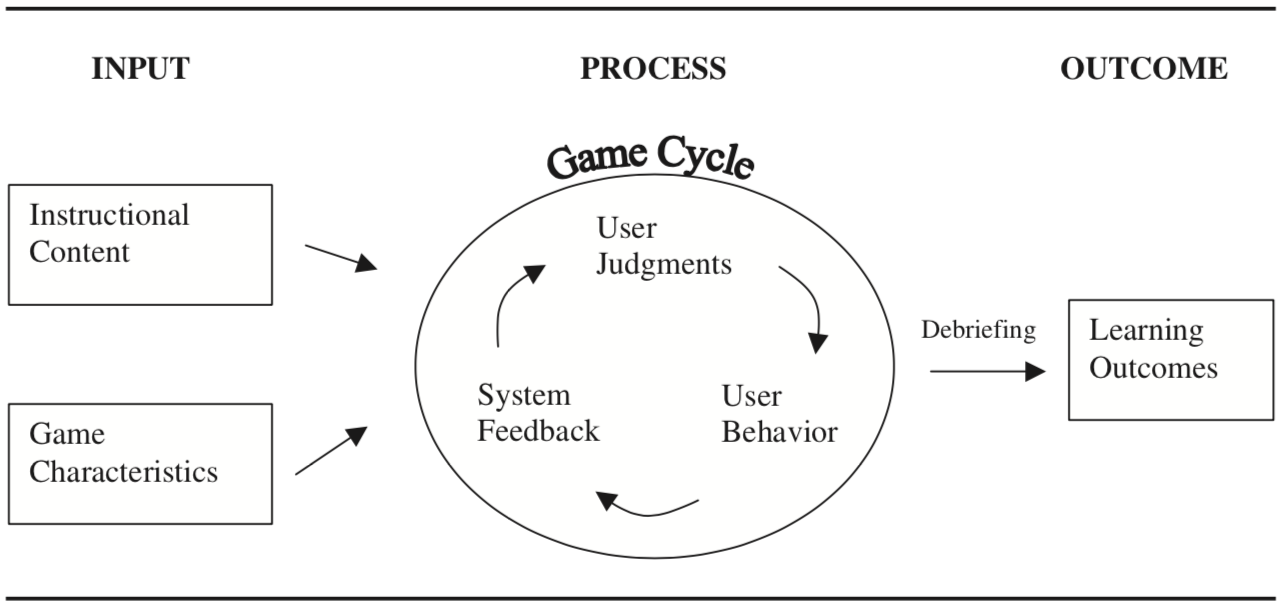
\includegraphics[width=1\textwidth]{Inputprocessoutcomegamemodel}
       \captionsetup{justification=centering}
\caption{Input-Process-Outcome Instructional Game Model  {\citep{Driskell2002}}}
\label{fig:Input_process_outcome_game_model}
\end{figure}

\subsection{Frameworks}

To be written.

EFM: A Model for Educational Game Design

Game object model version II: a theoretical framework for educational game development (318)

Game, motivation, and effective learning: An integrated model for educational game design (230)

Serious Games: A New Paradigm for Education?

\subsubsection{Game Genre}

To be written.

\subsection{Game Elements}

(CHANGE IT UP) \citeauthor{Barnes2007} ran a project that made University Students create games that would teach basic programming. They carried out evaluations to test participant learning from the game, and made some interesting observations as follows: Clear instructions and game goals must be provided and accessible throughout the game, Learning goals must be clearly tied to in-game feedback that motivates the player (through, e.g. experience points, health), and penalizes guessing, Humor can be a motivation for in-game interaction \citep{Barnes2007}.


\afterpage{\blankpage}

\chapter{Requirements Specification}
\afterpage{\blankpage}

\chapter{Design}
\afterpage{\blankpage}

\chapter{Implementation}
\afterpage{\blankpage}

\chapter{Testing}
\afterpage{\blankpage}

\chapter{Results}
\afterpage{\blankpage}

\chapter{Conclusions}
\afterpage{\blankpage}

\chapter{Future Work}
\afterpage{\blankpage}


\bibliography{litreview}
\addcontentsline{toc}{chapter}{Bibliography}


\appendix
\addtocontents{toc}{\protect\setcounter{tocdepth}{-1}}
\addtocontents{toc}{\protect\setcounter{tocdepth}{0}}
\appendixpage

\renewcommand\chaptername{Appendix}
%\chapter{Technical Specification and GA of the Skyseeker}\label{app:techspec}

\newpage
\chapter{Uncertainty Analysis} \label{app:errors}

\chapter{Screenshots} \label{app:screenshots}

\chapter{Ethics Checklist} \label{app:ethicschecklist}

\end{document}  